%\VignetteIndexEntry{1. Introduction to MultiDeconfounder}
%\VignetteKeywords{Software, Metagenomics, Microbiome, MultipleComparison, Metabolomics, Transcriptomics}
%\VignettePackage{MultiDeconfoundR}
%\VignetteEngine{knitr::knitr}

\pdfminorversion=5 
\pdfcompresslevel=9
\pdfobjcompresslevel=2


\documentclass{article}\usepackage[]{graphicx}\usepackage[usenames,dvipsnames]{color}
% maxwidth is the original width if it is less than linewidth
% otherwise use linewidth (to make sure the graphics do not exceed the margin)
\makeatletter
\def\maxwidth{ %
  \ifdim\Gin@nat@width>\linewidth
    \linewidth
  \else
    \Gin@nat@width
  \fi
}
\makeatother

\definecolor{fgcolor}{rgb}{0.251, 0.251, 0.251}
\newcommand{\hlnum}[1]{\textcolor[rgb]{0.816,0.125,0.439}{#1}}%
\newcommand{\hlstr}[1]{\textcolor[rgb]{0.251,0.627,0.251}{#1}}%
\newcommand{\hlcom}[1]{\textcolor[rgb]{0.502,0.502,0.502}{\textit{#1}}}%
\newcommand{\hlopt}[1]{\textcolor[rgb]{0,0,0}{#1}}%
\newcommand{\hlstd}[1]{\textcolor[rgb]{0.251,0.251,0.251}{#1}}%
\newcommand{\hlkwa}[1]{\textcolor[rgb]{0.125,0.125,0.941}{#1}}%
\newcommand{\hlkwb}[1]{\textcolor[rgb]{0,0,0}{#1}}%
\newcommand{\hlkwc}[1]{\textcolor[rgb]{0.251,0.251,0.251}{#1}}%
\newcommand{\hlkwd}[1]{\textcolor[rgb]{0.878,0.439,0.125}{#1}}%
\let\hlipl\hlkwb

\newenvironment{knitrout}{}{} % an empty environment to be redefined in TeX
\usepackage{alltt}



\RequirePackage[]{/home/tbirkne/R/x86_64-pc-linux-gnu-library/3.6/BiocStyle/resources/tex/Bioconductor}
\AtBeginDocument{\bibliographystyle{/home/tbirkne/R/x86_64-pc-linux-gnu-library/3.6/BiocStyle/resources/tex/unsrturl}}


%<<setup, echo=FALSE>>=
%suppressPackageStartupMessages({
%    library(BiocParallel)
%    library(BatchJobs)
%    library(VariantAnnotation)
%    library(GenomicAlignments)
%    library(RNAseqData.HNRNPC.bam.chr14)
%    library(TxDb.Hsapiens.UCSC.hg19.knownGene)
%})
%@

\usepackage{booktabs}
\usepackage{float}

\newcommand{\metadeconfoundR}{\Biocpkg{metadeconfoundR}}

\title{Introduction to \metadeconfoundR}
\author{Till Birkner\footnote{\url{tillb@online.de}}, Sofia K. Forslund}
\date{Edited: November 06, 2019; Compiled: \today}
\IfFileExists{upquote.sty}{\usepackage{upquote}}{}
\begin{document}

\maketitle

\tableofcontents

%%%%%%%%%%%%%%%%%%%%%%%%%%%%%%%%%%%%%%%%%%%%%%%%%%%%%%%%%%%%%%%%%%%%%%%%%%%%%
%%%%%%%%%%%%%%%%%%%%%%%%%%%%%%%%%%%%%%%%%%%%%%%%%%%%%%%%%%%%%%%%%%%%%%%%%%%%%
\section{Introduction}
%%%%%%%%%%%%%%%%%%%%%%%%%%%%%%%%%%%%%%%%%%%%%%%%%%%%%%%%%%%%%%%%%%%%%%%%%%%%%
%%%%%%%%%%%%%%%%%%%%%%%%%%%%%%%%%%%%%%%%%%%%%%%%%%%%%%%%%%%%%%%%%%%%%%%%%%%%%
%\packageVersion{BiocStyle::pkg_ver("metadeconfoundR")}
\Rpackage{metadeconfoundR} was developed to conduct confounder-aware biomarker analysis of large scale multi-omics datasets in parallel. This analysis is a two step process. 

First, significant associations between single omics features (like gut microbial OTUs) and metadata (like drug administration) are identified (fig\ref{fig:statistics}, left). Based on the data type of the respective metadata, either \Rcode{wilcox.test()} (for binary), \Rcode{cor.test()} (for continuous numerical) or \Rcode{kruskal.test()} (for neither numerical nor binary) is used. All three tests are rank-based to minimize assumptions about data distribution.
In addition to collecting p-values for all computed tests, effect size is measured if possible. In case of binary data, Cliff's Delta is computed by an algorithm based on the \Rcode{orddom::orddom()} function. For continuous data the ``estimate" component from \Rcode{cor.test()} is used. Since there is no effect size for categorical data with more than 2 levels, no value is reported here. It is recommended to introduce binary pseudo-variables for each level of the categorical metadata to circumvent this drawback.
    
\begin{figure}[H]
	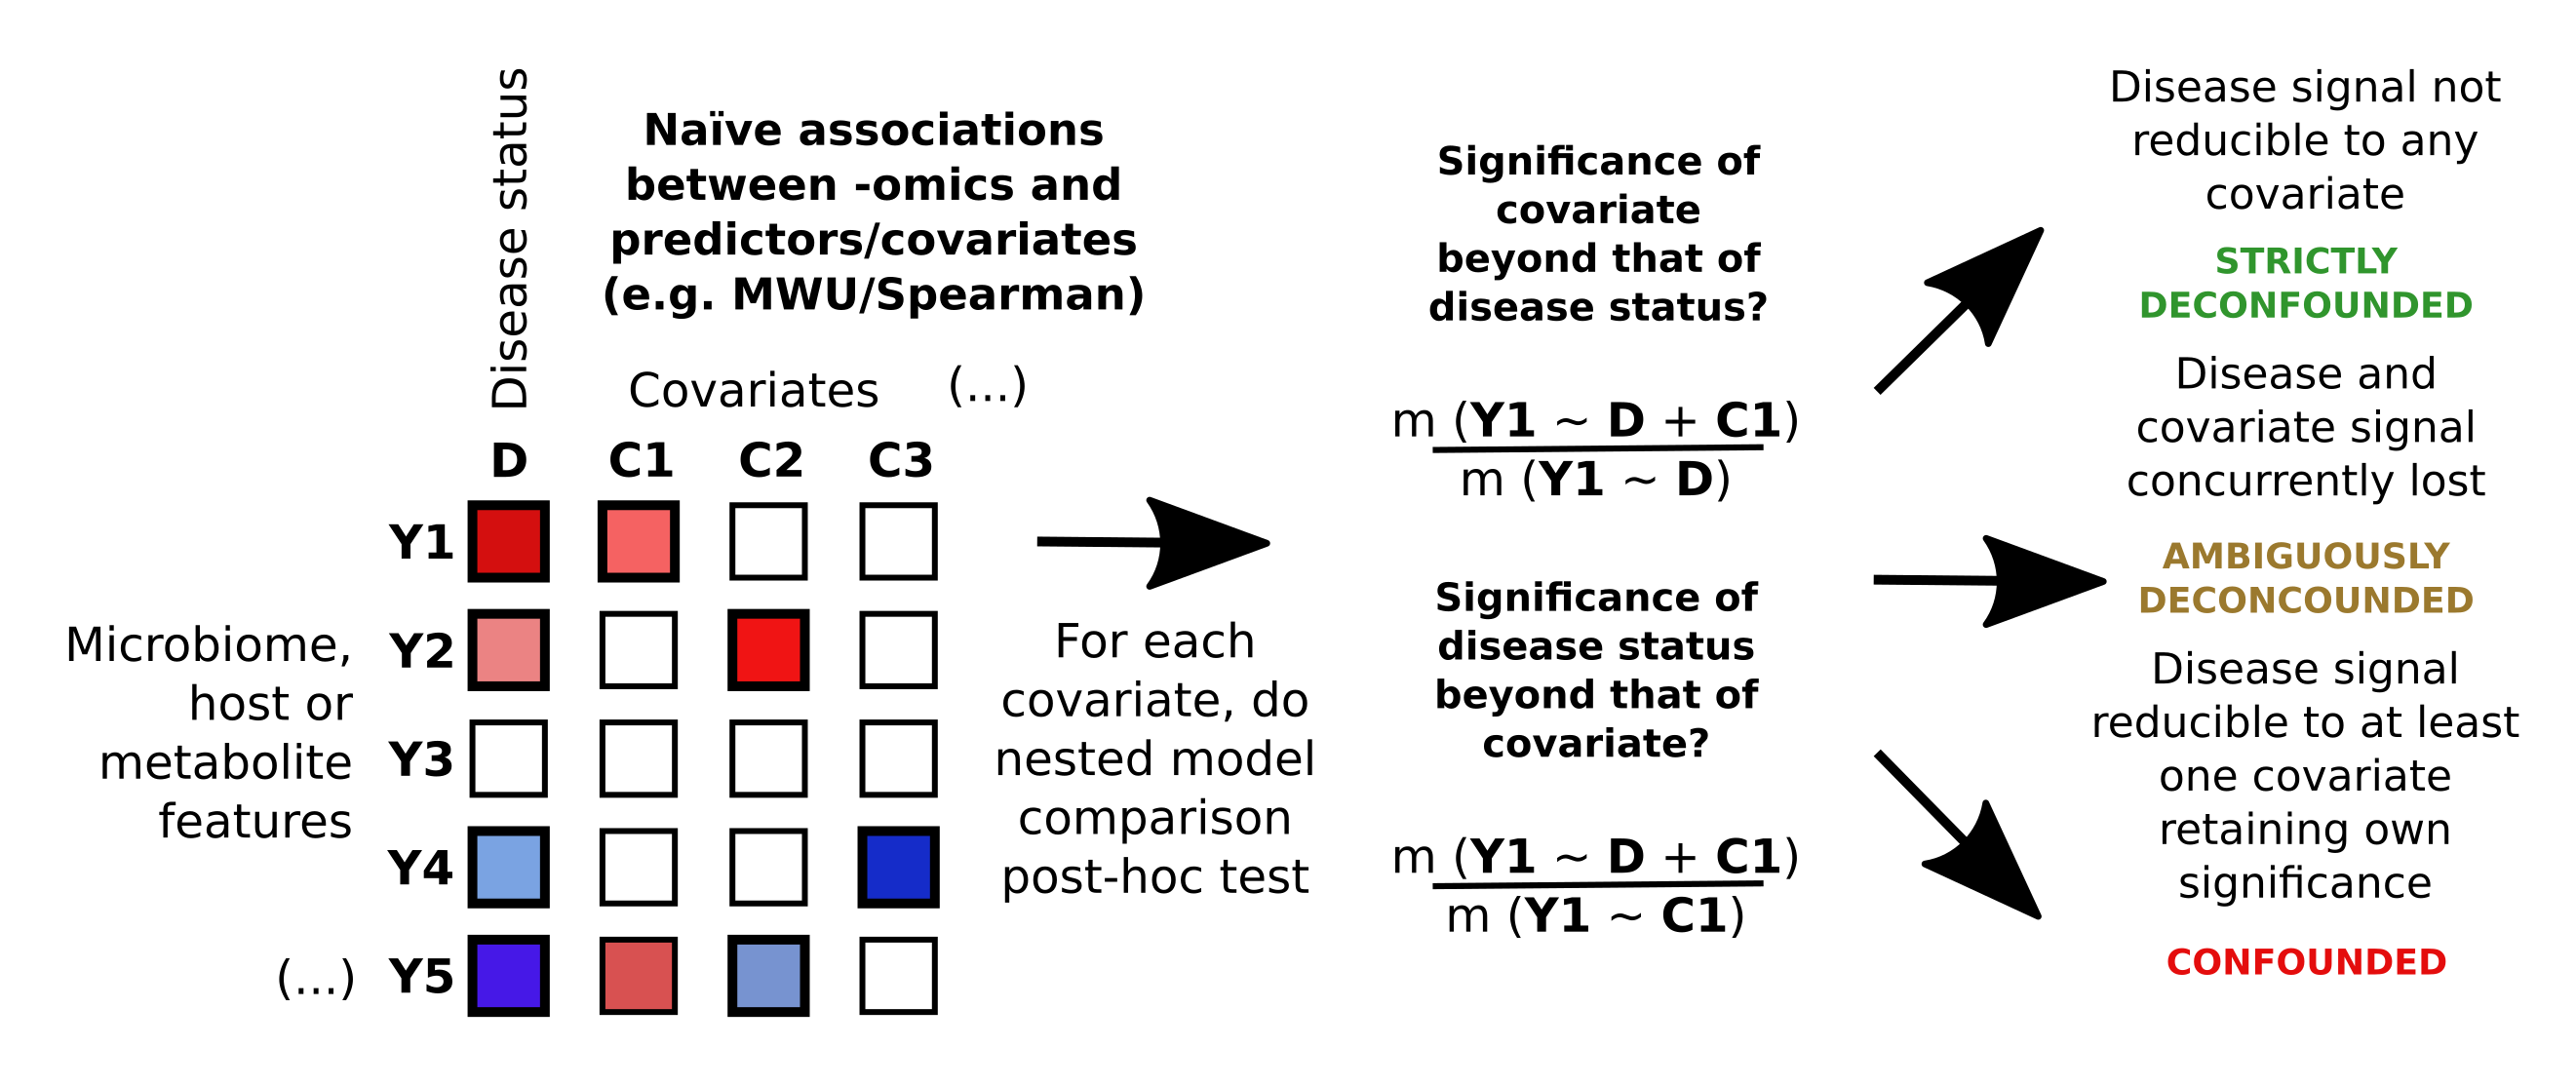
\includegraphics[width=\linewidth]{Figures/statistics.png}
	\caption{\bf Overview of main statistical approach used to determine confounding status.}
	(left) Each omics feature (Y) is independently tested for association to any of the predictors/covariates (D/C); Used test depends on data type of covariate. 
	(center) For each identified feature (Y1) $\leftrightarrow$ covariate (D/C) pair a set of linear models (either including an additional covariate or not) is fitted and a likelihood ratio is computed. 
	(right) Based on likelihood ratio a status for the feature (Y1) $\leftrightarrow$ covariate (D/C) pair is reported. Figure kindly provided by Sofia Forslund.
	\label{fig:statistics}
\end{figure}

\begin{figure}[H]
	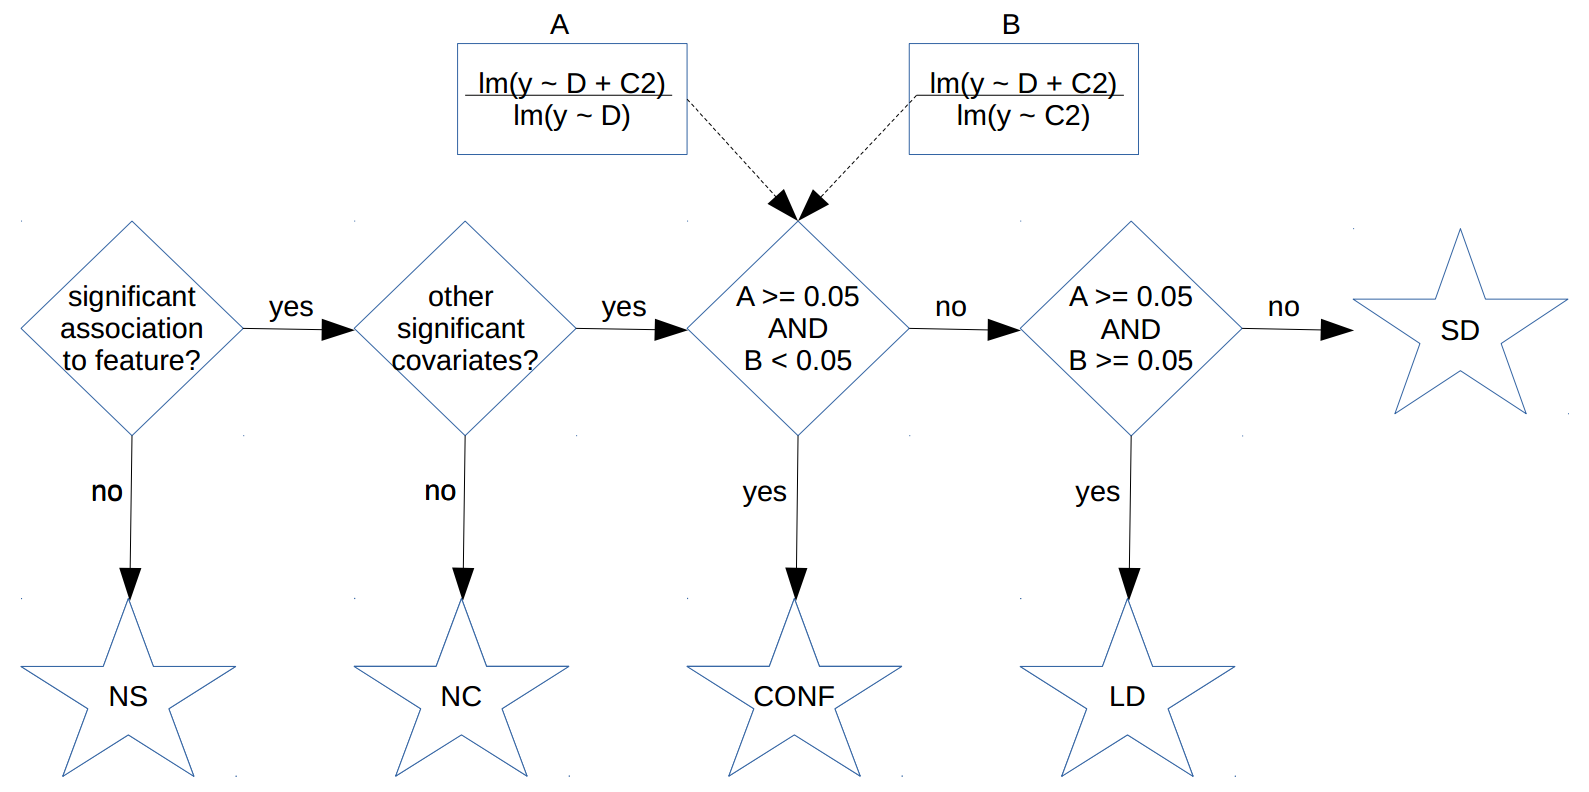
\includegraphics[width=\linewidth]{Figures/flowChartDecision.png}
	\caption{\bf Status labeling process in more detail.}
	For each feature $\leftrightarrow$ covariate combination these steps are done. A and B are the linear model likelihood ratios. Should there be more than one "other significant covariate" (C2), linear model likelihood ratio comparison has to be repeated for every single one of them. Whenever CONF is reached, the name of C2 is returned as label. Only when SD is reached for all C2, this will be returned as label.
	(y = feature, D = current covariate, C2 = other significant covariates, NS = not significant, NC = no covariates (i.e. trivially deconfounded), CONF = confounded, LD = laxly deconfounded, SD = strictly deconfounded)
	\label{fig:flowChart}
\end{figure}

In the second step, all hits are checked for confounding effects (fig \ref{fig:statistics}, center and right) and a status is reported for each feature $\leftrightarrow$  metadata combination (fig \ref{fig:flowChart}). A ``hit" here is defined as a feature $\leftrightarrow$ metadata association with small enough fdr-corrected p-value and big enough  effect size. Thresholds for both parameters can be set via \Rcode{QCutoff} and \Rcode{DCutoff} when starting the analysis. Since confounding of signal can only happen with more than one different metadata associated to a certain feature, all features with only one significant metadata are trivially deconfounded and get status ``No Covariates (NC)". \\
The actual confounder detection is done by a set of two likelihood ratio tests of nested linear models: For each feature with multiple covariates
 
 
 %For now please direct questions and bug reports to Till Birkner, a detailed introduction to the package will be added at a later stage.

%%%%%%%%%%%%%%%%%%%%%%%%%%%%%%%%%%%%%%%%%%%%%%%%%%%%%%%%%%%%%%%%%%%%%%%%%%%%%
%%%%%%%%%%%%%%%%%%%%%%%%%%%%%%%%%%%%%%%%%%%%%%%%%%%%%%%%%%%%%%%%%%%%%%%%%%%%%
\section{Quick start}
%%%%%%%%%%%%%%%%%%%%%%%%%%%%%%%%%%%%%%%%%%%%%%%%%%%%%%%%%%%%%%%%%%%%%%%%%%%%%
%%%%%%%%%%%%%%%%%%%%%%%%%%%%%%%%%%%%%%%%%%%%%%%%%%%%%%%%%%%%%%%%%%%%%%%%%%%%%

Install via tar.gz file: \Rcode{install.packages("metadeconfoundR\_0.1.1.tar.gz", repos = NULL)}
%The \Rpackage{MultideconfoundR} package is available at bioconductor.org
%and can be downloaded via \Rcode{BiocManager}:
%<<BiocManager, eval=FALSE>>=
%
%if (!requireNamespace("BiocManager", quietly = TRUE))
%    install.packages("BiocManager")
%BiocManager::install("MultideconfoundR")
%@
%
%Load \MultideconfoundR{}.
%<<MultideconfoundR>>=
%library(MultideconfoundR)
%@
%


%
%%%%%%%%%%%%%%%%%%%%%%%%%%%%%%%%%%%%%%%%%%%%%%%%%%%%%%%%%%%%%%%%%%%%%%%%%%%%%%
%%%%%%%%%%%%%%%%%%%%%%%%%%%%%%%%%%%%%%%%%%%%%%%%%%%%%%%%%%%%%%%%%%%%%%%%%%%%%%
\section{Use cases}
%%%%%%%%%%%%%%%%%%%%%%%%%%%%%%%%%%%%%%%%%%%%%%%%%%%%%%%%%%%%%%%%%%%%%%%%%%%%%%
%%%%%%%%%%%%%%%%%%%%%%%%%%%%%%%%%%%%%%%%%%%%%%%%%%%%%%%%%%%%%%%%%%%%%%%%%%%%%%

\begin{knitrout}
\definecolor{shadecolor}{rgb}{0.941, 0.941, 0.941}\color{fgcolor}\begin{kframe}
\begin{alltt}
\hlkwd{library}\hlstd{(metadeconfoundR)}

\hlkwd{data}\hlstd{(reduced_feature)}
\hlkwd{data}\hlstd{(metaMatMetformin)}

\hlstd{example_output} \hlkwb{<-} \hlkwd{MetaDeconfound}\hlstd{(}\hlkwc{featureMat} \hlstd{= reduced_feature,}
        \hlkwc{metaMat} \hlstd{= metaMatMetformin,}
        \hlkwc{nnodes} \hlstd{=} \hlnum{1}\hlstd{)}

\hlstd{knitr}\hlopt{::}\hlkwd{kable}\hlstd{(example_output}\hlopt{$}\hlstd{Ds[}\hlnum{1}\hlopt{:}\hlnum{3}\hlstd{,} \hlnum{1}\hlopt{:}\hlnum{5}\hlstd{],} \hlstr{"latex"}\hlstd{,} \hlkwc{digits} \hlstd{=} \hlnum{2}\hlstd{,} \hlkwc{booktabs} \hlstd{=} \hlnum{TRUE}\hlstd{)}
\end{alltt}
\end{kframe}
\begin{tabular}{lrrrrr}
\toprule
  & Status & Dataset & Metformin & continuous\_dummy & altered\_dummy\\
\midrule
MS0001 & -0.14 & Inf & -0.16 & 0.01 & 0.08\\
MS0006 & 0.20 & Inf & 0.13 & -0.02 & 0.13\\
MS0007 & 0.24 & Inf & 0.30 & 0.02 & -0.02\\
\bottomrule
\end{tabular}


\end{knitrout}

\begin{table}
	\caption{Summary of status assignments for each metadata variable}
	\label{tab:status_summary_unsplit}
\begin{knitrout}
\definecolor{shadecolor}{rgb}{0.941, 0.941, 0.941}\color{fgcolor}
\begin{tabular}{llllll}
\toprule
  &           Status & Dataset &   Metformin & continuous\_dummy & altered\_dummy\\
\midrule
 & altered\_dummy: 1 & NC:11 & Dataset: 1 & NS:50 & Dataset:18\\
 & Dataset      : 1 & NS: 2 & LD     : 2 & NA & NS     :29\\
 & LD           : 3 & SD:37 & NS     :32 & NA & SD     : 3\\
 & Metformin    : 1 & NA & SD     :12 & NA & NA\\
 & NC           : 1 & NA & Status : 3 & NA & NA\\
\addlinespace
 & NS           :26 & NA & NA & NA & NA\\
 & SD           :17 & NA & NA & NA & NA\\
\bottomrule
\end{tabular}


\end{knitrout}
\end{table}

\begin{table}
	\caption{Compostition of metadata ``Dataset"}
	\label{tab:Dataset_composition}
\begin{knitrout}
\definecolor{shadecolor}{rgb}{0.941, 0.941, 0.941}\color{fgcolor}
\begin{tabular}{rrr}
\toprule
CHN & MHD & SWE\\
\midrule
256 & 352 & 145\\
\bottomrule
\end{tabular}


\end{knitrout}
\end{table}

Cliff's Delta for categorical variables with more than two levels can't be computed and gets set to \Rcode{Inf}. By splitting up these variables into binary pseudo-variables will circumvent this. As can be seen in table \ref{tab:status_summary_unsplit}, status assignment is not affected by missing Cliff's Delta.
\begin{knitrout}
\definecolor{shadecolor}{rgb}{0.941, 0.941, 0.941}\color{fgcolor}\begin{kframe}
\begin{alltt}
\hlstd{example_output2} \hlkwb{<-} \hlkwd{MetaDeconfound}\hlstd{(}\hlkwc{featureMat} \hlstd{= reduced_feature,}
        \hlkwc{metaMat} \hlstd{= metaMatMetformin,}
        \hlkwc{nnodes} \hlstd{=} \hlnum{1}\hlstd{)}


\hlstd{knitr}\hlopt{::}\hlkwd{kable}\hlstd{(example_output2}\hlopt{$}\hlstd{Ds[}\hlnum{1}\hlopt{:}\hlnum{3}\hlstd{,} \hlnum{1}\hlopt{:}\hlnum{7}\hlstd{],} \hlstr{"latex"}\hlstd{,} \hlkwc{digits} \hlstd{=} \hlnum{2}\hlstd{,} \hlkwc{booktabs} \hlstd{=} \hlnum{TRUE}\hlstd{)}
\end{alltt}
\end{kframe}
\begin{tabular}{lrrrrrrr}
\toprule
  & Status & Metformin & continuous\_dummy & altered\_dummy & CHN & MHD & SWE\\
\midrule
MS0001 & -0.14 & -0.16 & 0.01 & 0.08 & -0.43 & 0.19 & 0.35\\
MS0006 & 0.20 & 0.13 & -0.02 & 0.13 & 0.12 & -0.49 & 0.67\\
MS0007 & 0.24 & 0.30 & 0.02 & -0.02 & 0.55 & -0.40 & -0.18\\
\bottomrule
\end{tabular}


\end{knitrout}

%%%%%%%%%%%%%%%%%%%%%%%%%%%%%%%%%%%%%%%%%%%%%%%%%%%%%%%%%%%%%%%%%%%%%%%%%%%%%
%%%%%%%%%%%%%%%%%%%%%%%%%%%%%%%%%%%%%%%%%%%%%%%%%%%%%%%%%%%%%%%%%%%%%%%%%%%%%
\section{\Rcode{sessionInfo()}}
%%%%%%%%%%%%%%%%%%%%%%%%%%%%%%%%%%%%%%%%%%%%%%%%%%%%%%%%%%%%%%%%%%%%%%%%%%%%%
%%%%%%%%%%%%%%%%%%%%%%%%%%%%%%%%%%%%%%%%%%%%%%%%%%%%%%%%%%%%%%%%%%%%%%%%%%%%%

\begin{kframe}
\begin{alltt}
\hlkwd{toLatex}\hlstd{(}\hlkwd{sessionInfo}\hlstd{())}
\end{alltt}
\end{kframe}\begin{itemize}\raggedright
  \item R version 3.6.1 (2019-07-05), \verb|x86_64-pc-linux-gnu|
  \item Locale: \verb|LC_CTYPE=en_US.UTF-8|, \verb|LC_NUMERIC=C|, \verb|LC_TIME=de_DE.UTF-8|, \verb|LC_COLLATE=en_US.UTF-8|, \verb|LC_MONETARY=de_DE.UTF-8|, \verb|LC_MESSAGES=en_US.UTF-8|, \verb|LC_PAPER=de_DE.UTF-8|, \verb|LC_NAME=C|, \verb|LC_ADDRESS=C|, \verb|LC_TELEPHONE=C|, \verb|LC_MEASUREMENT=de_DE.UTF-8|, \verb|LC_IDENTIFICATION=C|
  \item Running under: \verb|Ubuntu 18.04.3 LTS|
  \item Matrix products: default
  \item BLAS:   \verb|/usr/lib/x86_64-linux-gnu/openblas/libblas.so.3|
  \item LAPACK: \verb|/usr/lib/x86_64-linux-gnu/libopenblasp-r0.2.20.so|
  \item Base packages: base, datasets, graphics, grDevices, methods,
    stats, utils
  \item Loaded via a namespace (and not attached):
    BiocManager~1.30.8, BiocStyle~2.12.0, compiler~3.6.1,
    digest~0.6.21, evaluate~0.14, htmltools~0.4.0, knitr~1.25,
    magrittr~1.5, Rcpp~1.0.2, rlang~0.4.0, rmarkdown~1.16,
    stringi~1.4.3, stringr~1.4.0, tools~3.6.1, xfun~0.10, yaml~2.2.0
\end{itemize}


\end{document}
